\section{Model}\label{sec:model}
This section presents a mathematical framework for online scheduling in LLM inference under memory constraints. 

\subsection{Prompts and Inference Process}

We analyze a system designed to process user queries, referred to as \textit{prompts}, utilizing a single Graphics Processing Unit (GPU) for computation. We focus on maximizing the utilization of single GPU and avoid the communication costs associated with multi-GPU systems. Each prompt is divided into discrete units known as \textit{tokens} during the prefill phase and generates output text through an inference process in the decode phase. A token represents a distinct text element, such as a word or subword, and its processing relies on a memory structure called the Key-Value (KV) cache. As noted in the introduction, the KV cache improves inference efficiency significantly by storing the computational history of prior tokens, thus avoiding redundant computations. The cache size increases as tokens are processed, requiring careful memory management to maintain system performance.

% A Central Processing Unit (CPU) with unlimited memory acts as auxiliary storage; however, transferring a token’s KV cache from the CPU to the GPU introduces a delay \( d_s > 0 \) per token.

% \textbf{Prompt Characteristics}: Prompts arrive stochastically and are classified into \( m \) distinct types, indexed by \( j \in \{1, \dots, m\} \). A prompt of type \( j \) has the following properties:
% \[
% \begin{cases}
% \text{a length of } l_j \text{ tokens after completing the prefill phase;} \\
% \text{a length of } l_j + l_j' \text{ tokens after completing the decode phase.}
% \end{cases}
% \]
% We assume that prompts of type \( j \) follow a Poisson process with a rate of \( \lambda_j \).

% \gan{I will add more explanation. The rate $\lambda_j$ comes from the real world inference serving data, and the rate of one type is indeed the sum of rates of many mini types in the real world inference serving data. Or maybe this part should add to the nested WAIT section?}

\textbf{Prompt Characteristics}: Prompts arrive stochastically and are classified into \( m \) distinct types, indexed by \( j \in \{1, \dots, m\} \). A prompt of type \( j \) has the following properties:
\[
\begin{cases}
\text{a length of } l_j \text{ tokens after completing the prefill phase;} \\
\text{a length of } l_j + l_j' \text{ tokens after completing the decode phase.}
\end{cases}
\]
We assume that prompts of type \( j \) follow a Poisson process with a rate of \( \lambda_j \). In practice, these types allow us to cluster prompts with varying output lengths into a manageable number of categories. Specifically, even though prompts may have different output lengths (i.e., different \( l_j' \)), we group them into type \( j \) by adjusting the arrival rate \( \lambda_j \) and the representative output length \( l_j' \) for that cluster. The rate \( \lambda_j \) is derived from real-world inference serving data and represents the aggregated arrival rates of multiple sub-types with similar characteristics. This clustering approach ensures that the model remains tractable while capturing the diversity of prompt behaviors. Furthermore, our algorithm and theoretical results do not depend on the number of types \( m \), but rather on the total arrival rates across all types. This dependence on total arrival rates ensures that our approach scales effectively and remains robust across different operational scenarios, regardless of how many types are defined.

The inference process for a prompt of type \( j \) comprises two sequential phases:
\begin{enumerate}
    \item \textbf{Prefill Phase}: The system initializes the KV cache for the \( l_j \) input tokens in a single batch iteration.  
    % For memory-intensive prompts, the input sequence may be divided into smaller \textit{chunks} of size \( k \leq l_j \), processed sequentially to optimize memory usage.
    
    \item \textbf{Decode Phase}: After prefill, the system generates one token  per iteration in decode phase. Each new token updates the KV cache and consumes additional memory, requiring \( l_j' \) iterations (stages) to complete the decoding. When the prompt complete the decoding, the KV cache memory will be cleared from the GPU.
\end{enumerate}
For simplicity, we designate prompts in the prefill phase as being in \textit{stage 0} and prompts at the \( k \)-th iteration of the decode phase as being in \textit{stage \( k \)}. This notation captures the progression of prompts through the inference process, where stage 0 represents the initial prefill phase, during which the input KV cache is computed, and stages \( k = 1, 2, \dots \) correspond to the iterations of output tokens in the decode phase.

To further illustrate this process, consider the example in Figure \ref{fig:intro_example}. The prompt ``Is apple a fruit?'' is tokenized into a sequence of five tokens during the prefill phase (stage 0). The system then computes the KV cache, requiring five memory units to store the intermediate representations. Upon completion of the prefill phase, the prompt transitions to the decode phase at stage 0, signifying that it is fully prefilled and prepared for the generation of subsequent tokens.

During the decode phase, the prompt at stage 0 is added to a batch, which may include other prompts in either the prefill or decode phases. At this stage, the memory contribution of the prompt to the batch is five units. After one iteration of batch inference, the prompt generates a new token and advances to stage 1, increasing its memory consumption to six units.

This process continues iteratively. When the prompt reaches stage 4, it has generated its final token, and the memory consumption of its KV cache reaches nine units. Upon detecting the ``End of Sequence'' (EOS) token, the system clears the KV cache, completing the inference for this prompt.

\subsection{Batching and Processing Time}
To optimize resource utilization, the GPU processes tasks in \textit{batches}, combining prompts for prefilling and prefilled prompts for decoding. Figure \ref{fig:batching_example} provides an illustrative example.

Consider a batch composed of:
\begin{itemize}
    \item \( n_1 \) prompts in the prefill phase, each with an input length of \( k_i \) tokens for \( i = 1, 2, \dots, n_1 \). These prompts are processed to initialize their KV caches.
    \item \( n_2 \) prompts in the decode phase, each with output length of \( s_i = l_{j(i)} + k_i \) tokens after the current iteration, where \( l_{j(i)} \) is the input length of prompt \( i \) of type \( j(i) \), and \( k_i \) denotes the number of tokens generated so far in the decode phase for prompt \( i \).
\end{itemize}


\begin{figure}[h]
    \centering
    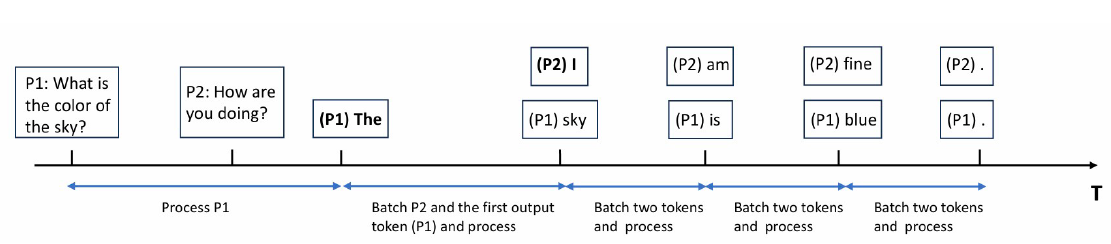
\includegraphics[width=1\linewidth]{fig_batching.png}
    \caption{Example of batching and scheduling \citep{jaillet2025onlineschedulingllminference}.}
    \label{fig:batching_example}
\end{figure}

Based on experimental results from \cite{agrawal2023sarathi,kwon2023efficient,zhong2024distserve}, we model the \textit{iteration time} to process a batch as:
\begin{equation}
\label{eq:time_consump}
    \tau = d_0 + d \cdot \left( \sum_{i=1}^{n_1} k_i + \sum_{i'=1}^{n_2} s_{i'} \right),
\end{equation}
where \( d_0 \) denotes the fixed overhead time associated with processing a batch, and \( d \) represents the time cost per unit of memory. This formulation indicates that the iteration time for each batch scales linearly with the total memory utilization, reflecting the direct dependence of computational latency on memory consumption involving reading existing KV cache and computing the new one.
% \begin{equation}
% \label{eq:time_consump}
%     \tau = \max \left\{ d_{0f} + d_f \cdot \max_{i=1}^{n_1} \{ k_i \}, \; d_{0c} + d_c \cdot \sum_{i=1}^{n_2} s_i \right\},
% \end{equation}
% where:
% \begin{itemize}
%     \item \( d_{0f} \) and \( d_{0c} \) denote constant processing times for forward propagation operations, encompassing linear layers and related computations.
%     \item \( d_f \) represents the prefill processing time per token.
%     \item \( d_c \) represents the decode processing time per token. Typically, \( d_f, d_{0f} \ll d_c s_i \), indicating that decode time dominates when \( n_2 > 0 \). For this study, we assume \( \tau = d_{0c} + d_c \cdot \sum_{i=1}^{n_2} s_i \) whenever \( n_2 > 0 \).
% \end{itemize}

% \gan{We do not need very clear explanation! Need add explanation on the time consumption of "read" the KV cache on GPU and the prompt for prefill on CPU?}


\subsection{Constraints and Performance Metrics}

\textbf{Memory Constraint}: At any time \( t \), the total memory occupied by \textit{active prompts}---prompts that have begun processing on the GPU but have not yet completed their inference---must not exceed the GPU's memory capacity \( C \). Consider a batch \( B^t \) at time \( t \), comprising prompts where the \( i \)-th prompt is of type \( j^t(i) \) with memory usage \( l_{j^t(i)} + k_i^t \). Here, \( l_{j^t(i)} \) represents the input length (number of tokens in the prompt), and \( k_i^t \in \{0, 1, \dots, l_{j^t(i)}'\} \) indicates the processing stage of the \( i \)-th prompt, resulting in an output length of \( l_{j^t(i)} + k_i^t \) after the current iteration.

The memory constraint ensures that the cumulative memory usage of all active prompts, including those in the current batch and any incomplete prompts from previous batches, stays within the GPU's capacity. This is formally defined as:
\[
\sum_{i=1}^{B^t} (l_{j^t(i)} + k_i^t) \leq C \quad \forall t.
\]
This limitation is critical to prevent memory overflow, ensuring system stability throughout the processing timeline.

\textbf{Performance Metrics}: The efficiency and responsiveness of the system are assessed through the following metrics:
\begin{itemize}
    \item \textit{Time to First Token (TTFT\(^t\))}: The average duration from a prompt's arrival to the generation of its first output token of decode phase, measuring initial response speed up to time \( t \).
    \item \textit{Latency\(^t\)}: The average total time from a prompt's arrival to the completion of all \( l_{j^t(i)}' \) output tokens, capturing the overall task completion time up to time \( t \).
    \item \textit{Throughput\(^t\)}: The average total number of output tokens generated per unit time, reflecting the system's workload capacity up to time \( t \). We only count a prompt's output when it completes in order to avoid repeatedly process the same short prompt for generating higher throughput.
\end{itemize}

\subsection{Problem Formulation}

We define \( \Pi \) as the set of all non-preemptive admissible online scheduling policies. These policies make decisions based solely on historical information, aiming to maximize the average throughput over a time horizon \( T \), while ensuring that the average Time to First Token (TTFT) and latency satisfy predefined thresholds. Formally, the optimization problem is expressed as:

\[
\begin{aligned}
\max_{\pi \in \Pi} \quad & \mathbb{E} \left[ \throughput^T \right] \\
\text{subject to} \quad & \mathbb{E} \left[ \textbf{TTFT}^T \right] \leq F^T, \\
& \mathbb{E} \left[ \textbf{Latency}^T \right] \leq L^T, \\
& \sum_{i=1}^{B^t} \left( l_{j^t(i)} + k_i^t \right) \leq C \quad \forall t,
\end{aligned}
\]

where \( F^T \) and \( L^T \) represent specified thresholds that guarantee a responsive user experience. This formulation encapsulates the trade-offs between resource efficiency and service quality, establishing a foundation for designing effective scheduling policies in subsequent sections.

